\begin{frame}{\og{}Napoléon des névroses \fg{} ou \og{}Paganini de l'hystérie\fg{} {\footnotesize(\hypersetup{citecolor=yellow}\cite{marmion2015freud})}}

{\textsc{Jean-Martin Charcot (1825-1893)}}
%\hbox{\hspace{25em} 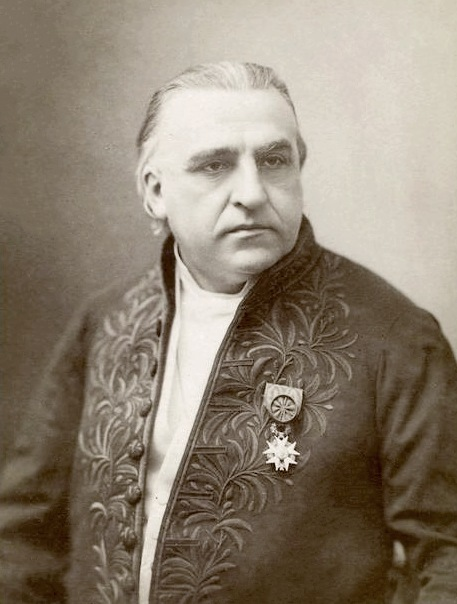
\includegraphics[scale=0.07]{pic/Jean-Martin_Charcot.jpg}}
%\\{\scriptsize Portrait de\\Charcot (\href{https://fr.wikipedia.org/wiki/Jean-Martin_Charcot}{Wikipedia}).}
\hbox{\hspace{6em} 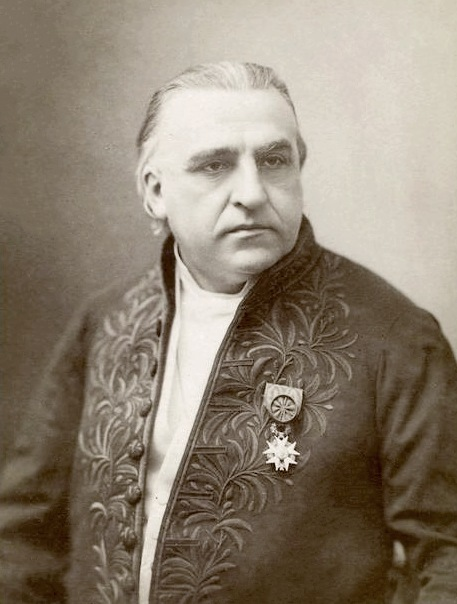
\includegraphics[scale=0.06]{pic/Jean-Martin_Charcot.jpg}}\\\hbox{\hspace{23.3em}{\tiny Source : \href{https://fr.wikipedia.org/wiki/Jean-Martin_Charcot}{Wikipedia}}.}
\begin{itemize}
\item père de la neurologie moderne et française au XIX\ieme{} s. 
\item leçons cliniques du mardi à l'hôpital de la Salpêtrière à Paris \\
\begin{flushright}
\small\leftguillemet{} Mecque de la neurologie \rightguillemet{}
\end{flushright}
\end{itemize}
\begin{enumerate}[\indent {}]
\item Contributions majeures :
	\begin{itemize}
	    \item hystérie : résultat d'une lésion dynamique des circuits cérébraux
    \item hypnose : analyse des symptômes hystériques et outil thérapeutique
    \item SEP\footnote{abbr. \textit{sclérose en plaques}.} disséminée (description) $\rightarrow$ sclérose multiple
    \item SLA\footnote{abbr. \textit{sclérose latérale amyotrophique}.} (description) $\rightarrow$ maladie de Charcot / Lou Gehrig
    \item maladie de Parkinson : concepteur du terme (avec A. Vulpian)
	\end{itemize}  
	\end{enumerate}
    % \item hystérie est due à une \textit{lésion dynamique} de l’encéphale, liée à un traumatisme de nature physique (accident de train, chute, choc$\dots$) -- possible de recréer sous hypnose
    % \item impact sur les acteurs dans ou en dehors de sa discipline : S. Freud, G. de la Tourette, E. Zola$\dots$
    \begin{flushright}
{\footnotesize(\cite{camargo2024jean})}
\end{flushright}

%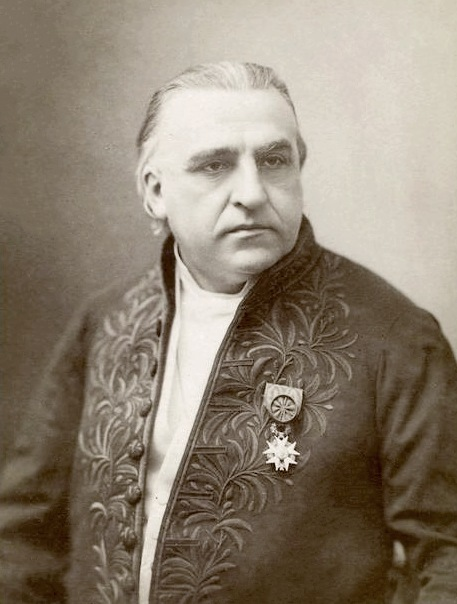
\includegraphics[width=10pt]{pic/Jean-Martin_Charcot.jpg}%
%\\{\scriptsize Portrait de\\Charcot (\href{https://fr.wikipedia.org/wiki/Jean-Martin_Charcot}{Wikipedia}).}



\end{frame}
